% Created 2023-04-06 Thu 00:06
% Intended LaTeX compiler: pdflatex
\documentclass[a4paper,twocolumn]{article}
\usepackage[utf8]{inputenc}
\usepackage[T1]{fontenc}
\usepackage{graphicx}
\usepackage{longtable}
\usepackage{wrapfig}
\usepackage{rotating}
\usepackage[normalem]{ulem}
\usepackage{amsmath}
\usepackage{amssymb}
\usepackage{capt-of}
\usepackage{hyperref}
\usepackage[T1]{fontenc}
\usepackage{tgbonum}
\usepackage{biblatex}
\addbibresource{/home/dp/Documents/Research_paper_SFR/bibl/bibliography/bibliography.bib}
\usepackage{amsmath}
\usepackage{graphicx}
\usepackage{caption}
\usepackage{booktabs}
\usepackage{hyperref}
\let\description\compactdesc
\raggedbottom
\date{\today}
\title{Finding Adel}
\hypersetup{
 pdfauthor={},
 pdftitle={Finding Adel},
 pdfkeywords={},
 pdfsubject={},
 pdfcreator={Emacs 28.2 (Org mode 9.6.1)}, 
 pdflang={English}}
\begin{document}

\maketitle
According to P. Kroupa et al. 2020\autocite{kroupaConstraintsStarFormation2020} current star formation rates of galaxies can be described by the 'delayed-\(\tau\)' model as


\begin{equation} \label{eq:SFR}
SFR_{0,del}=\frac{A_{del}xe^{-x}}{\tau},\text{ where } x=\frac{t_{sf}}{\tau}
\end{equation}

\noindent
where \(\tau\) is the star formation time-scale,  \(t_{sf}\) is the real time of star formation in a given galaxy and \(A_{del}\) a normalization constant.

For a galaxy that forms stars from the time t\textsubscript{1} to t\textsubscript{2}=the pressent day (if the galaxy is still forming stars) the SFH can be written as \(SFR(t) = \overline{SFR}+\Delta SFR(t)\), such that the average SFR of the galaxy can be witten as

\begin{equation}\label{eq:int of av_SFR}
\overline{SFR} = \frac{1}{t_{sf}} \left(\int^{t_2}_{t_1}\overline{SFR}dt+ \int^{t_2}_{t_1}\Delta SFR(t)\right)
\end{equation}
with temporal deviations from \(\overline{SFR}\) satisfying:

$$\int^{t_2}_{t_1} \Delta SFR dt = 0M_\odot$$

So from the equations (\ref{eq:SFR}) and (\ref{eq:int of av_SFR}) we get the averge SFR:

\begin{equation}\label{eq:av_SFR-x}
\overline{SFR_{del}}=\frac{A_{del}}{t_{sf}}[1-(1+x)e^{-x}]
\end{equation}
and can also be defined by the present day stellar mass

\begin{equation}\label{eq:av_SFR M*}
    \overline{SFR}=\frac{\zeta M_*}{t_{sf}}
\end{equation}
\noindent where \(\zeta\) accommodates for mass-loss through stellar evolution and \(\zeta\approx 1.3\).

From the equations (\Ref{eq:int of av_SFR}) and (\ref{eq:av_SFR-x}) we can derive that the \(A_{del}\) must be independent from the time/ constant throughout the life of the galaxy.

Also from the equation (\ref{eq:SFR}) we can find the units of the \(A_{del}\)
\begin{equation} \label{eq:units}
\begin{align}
\left[SFR_{0,del}\right]&=\frac{\left[A_{del}\right]\left[x\right]\left[e^{-x}\right]}{\left[\tau\right]}\\
\frac{[M_*]}{[time]}& = \frac{[A_{del}]\cdot 1\cdot 1}{[time]}\\
[M_*]& = [A_{del}]
\end{align}
\end{equation}

So we can expect that the \(A_{del}\) can be expressed as
\begin{equation}\label{eq:A=f(M)}
A_{del}=c\cdot M \Leftrightarrow \log(A_{del})= log(M)+log(c)
\end{equation}
\noindent where c is a constant and M the stellar mass (\(M_*\)), the gas mass (\(M_g\)) or the total mass of galaxy(\(M_t = M_* + M_g\)).

The equations (\ref{eq:SFR}) and (\ref{eq:av_SFR-x}) create a system of 2 equations and 3 variables (the SFR and the stellar masses are given), since A\textsubscript{del} has never been calculated

\section{Constant \(t_{sf}\)}
\label{sec:orge82f914}

The observed ages of galactic discs are \(t_{sf}\approx 12\) Gyr\autocite{knoxSurveyCoolWhite1999}, so we assume an approximation of \(t_{sf}=12.5\) Gyr. Having one out of the three variables as a constant we can calculate the \(A_{del}|_{t_{sf}}\) and \(\tau|_{t_{sf}}\) and plot them (figures \ref{fig:A-x_tsf} and \ref{fig:A-tau_tsf}).

\begin{figure}[!htpb]
\centering
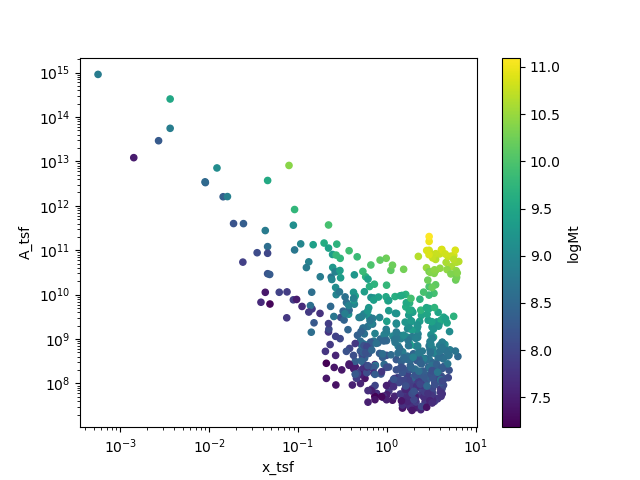
\includegraphics[width=.9\linewidth]{./figs/x-A_tsf.png}
\caption{\label{fig:A-x_tsf}\(A_{del} = f(x)\) for constant t\textsubscript{sf}}
\end{figure}

\begin{figure}[!htpb]
\centering
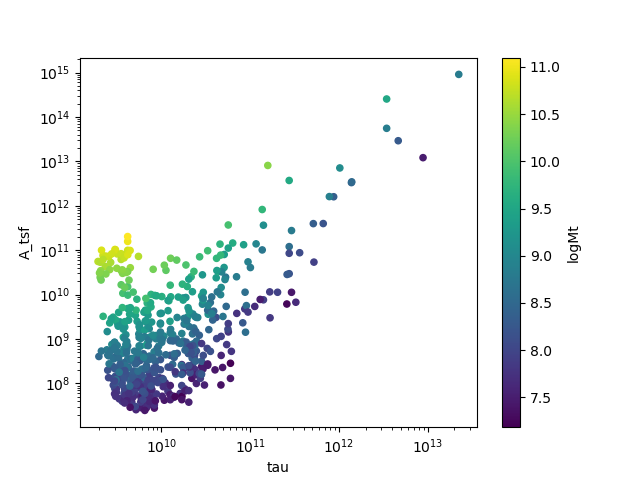
\includegraphics[width=.9\linewidth]{./figs/T-A_tsf.png}
\caption{\label{fig:A-tau_tsf}\(A_{del} = f(\tau)\) for constant t\textsubscript{sf}}
\end{figure}

\section{Constant \(\tau\)}
\label{sec:org8d5bda4}

Now assuming for a constant \(\tau = 3.5\) Gyr the system can again be solved numerically for each galaxy and the values of \(A_{del}|_{\tau}\) and \(t_{sf}|_{\tau}\) can be found and plotted (figures \ref{fig:A-x_tau} and \ref{fig:A-tsf_tau}).

\begin{figure}[!htpb]
\centering
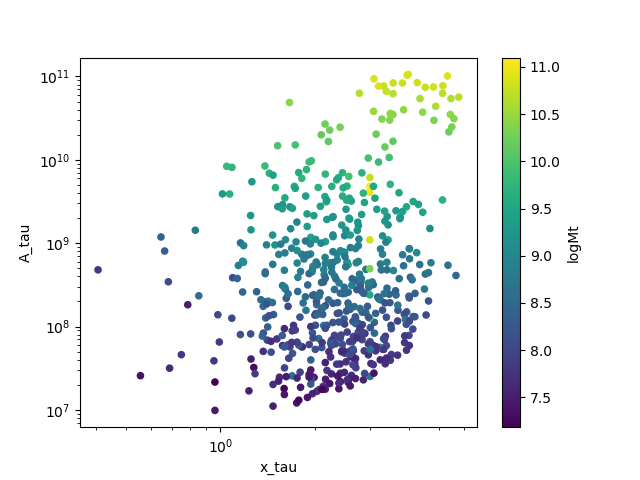
\includegraphics[width=.9\linewidth]{./figs/x-A_tau.png}
\caption{\label{fig:A-x_tau}\(A_{del} = f(x)\) for constant \(\tau\)}
\end{figure}

\begin{figure}[!htpb]
\centering
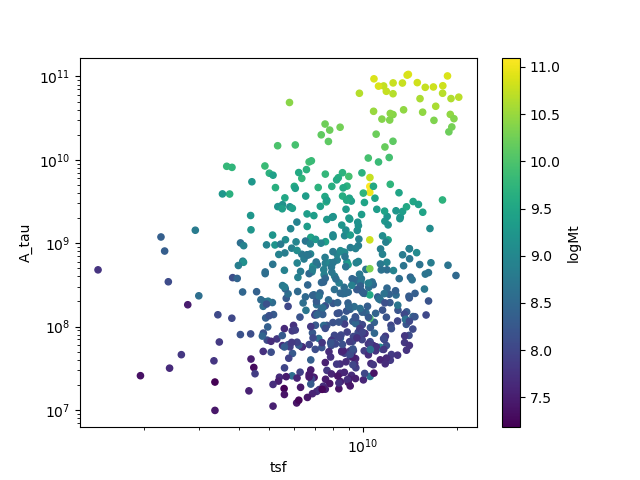
\includegraphics[width=.9\linewidth]{./figs/T-A_tau.png}
\caption{\label{fig:A-tsf_tau}\(A_{del} = f(t_{sf})\) for constant \(\tau\)}
\end{figure}

\section{Finding the \(A_{del} = f(\text{Mass})\) relation}
\label{sec:orgb5ebed2}

If we plot the \(A_{del}\) with the 3 given masses of each galaxy, both for a constant \(\tau\) and a constant \(t_{sf}\), we observe that indeed there is a correlation in the form of:
$$
\log(A_{del}) = c_1\log(\text{Mass})+c_2
$$

\begin{enumerate}
\item For a constant \(t_{sf}\) the correlations are:
\begin{enumerate}
\item Total mass: \(R^2=48\%\) (Fig. \ref{fig:A_tsf_Mt})
\item Mass of the Gasses: \(R^2=43\%\) (Fig. \ref{fig:A_tsf_Mg})
\item Stellar Mass: \(R^2=44\%\) (Fig. \ref{fig:A_tsf_StellarMass})
\end{enumerate}

\item For a constant \(\tau\) the correlations are:
\begin{enumerate}
\item Total mass: \(R^2=91\%\) (Fig. \ref{fig:A_tau_Mt})
\item Mass of the Gasses: \(R^2=70\%\) (Fig. \ref{fig:A_tau_Mg})
\item Stellar Mass: \(R^2=90\%\) (Fig. \ref{fig:A_tau_StellarMass})
\end{enumerate}
\end{enumerate}

In both cases the best correlation is  \(A_{del} = f(M_t)\) and for \(\tau =\) const. the correlation is excelent.
\begin{equation}\label{eq:logMt-log_A_tsf-color_x_tsf}
\log(A_{del}|_t_{sf}) = (9.6(4) \times 10^{-1})\cdot \log(M_t) + (8(4) \times 10^{-1})
\end{equation}
\begin{equation}\label{eq:logMt-log_A_tau-color_x_tau}
\log(A_{del}|_\tau) = (1.025(14) \times 10^{0})\cdot \log(M_t) + (-3.0(1.2) \times 10^{-1})
\end{equation}

For both equations (\ref{eq:logMt-log_A_tsf-color_x_tsf}) and (\ref{eq:logMt-log_A_tau-color_x_tau}) \(c_1\approx 1\) so they fit the equation (\ref{eq:A=f(M)}).

\begin{figure}[!htpb]
\centering
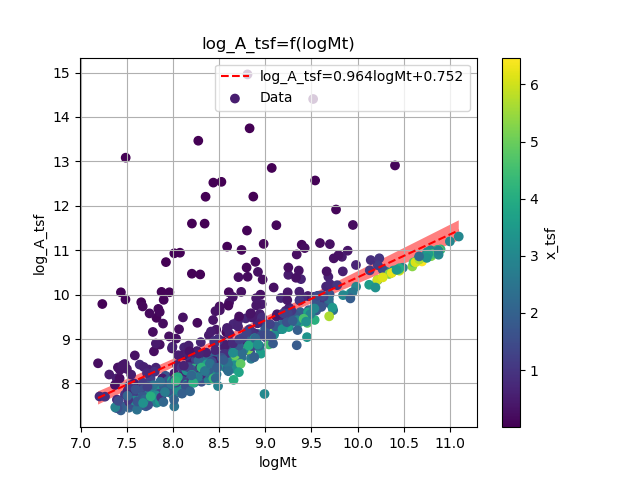
\includegraphics[width=.9\linewidth]{./figs/logMt-log_A_tsf-color_x_tsf.png}
\caption{\label{fig:A_tsf_Mt}Total Mass \(M_t\) - \(A_{del}|_{t_{sf}}\)}
\end{figure}

\begin{figure}[!htpb]
\centering
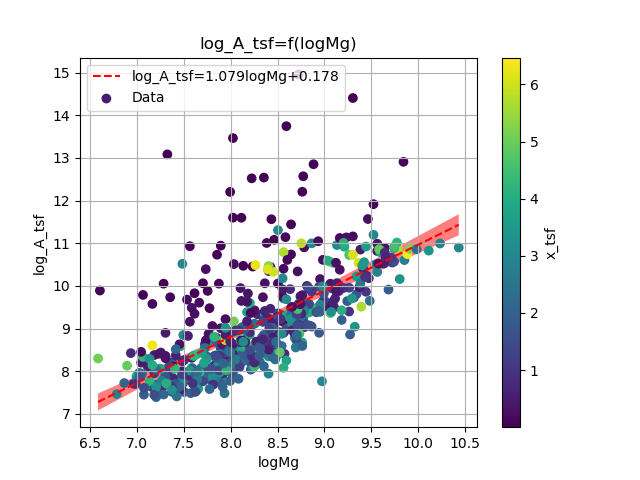
\includegraphics[width=.9\linewidth]{./figs/logMg-log_A_tsf-color_x_tsf.png}
\caption{\label{fig:A_tsf_Mg}Mass of the gasses \(M_g\) - \(A_{del}|_{t_{sf}}\)}
\end{figure}

\begin{figure}[!htpb]
\centering
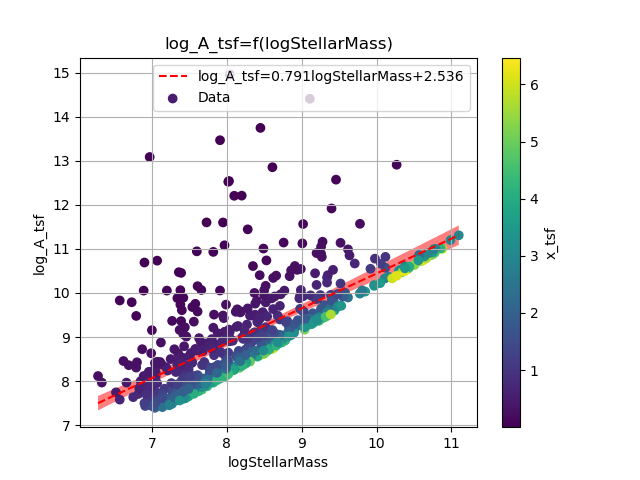
\includegraphics[width=.9\linewidth]{./figs/logStellarMass-log_A_tsf-color_x_tsf.png}
\caption{\label{fig:A_tsf_StellarMass}Stellar Mass \(M_*\) - \(A_{del}|_{t_{sf}}\)}
\end{figure}

\begin{figure}[!htpb]
\centering
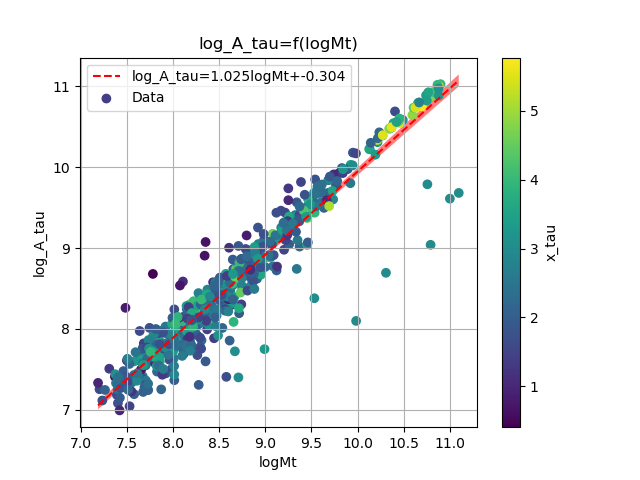
\includegraphics[width=.9\linewidth]{./figs/logMt-log_A_tau-color_x_tau.png}
\caption{\label{fig:A_tau_Mt}Total Mass \(M_t\) - \(A_{del}|_{\tau}}\)}
\end{figure}

\begin{figure}[!htpb]
\centering
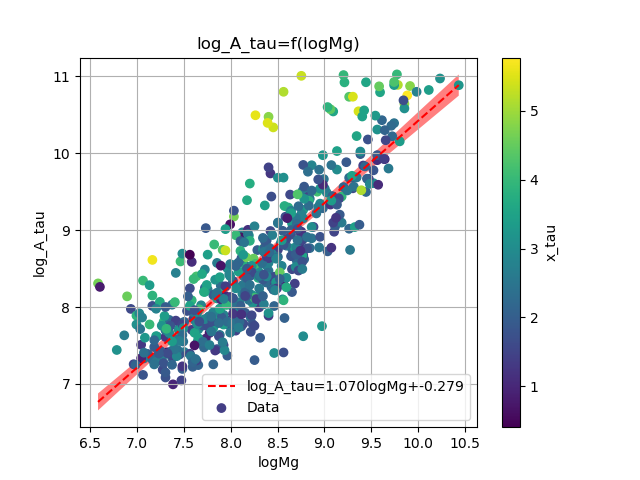
\includegraphics[width=.9\linewidth]{./figs/logMg-log_A_tau-color_x_tau.png}
\caption{\label{fig:A_tau_Mg}Mass of the gasses \(M_g\) - \(A_{del}|_{\tau}\)}
\end{figure}

\begin{figure}[!htpb]
\centering
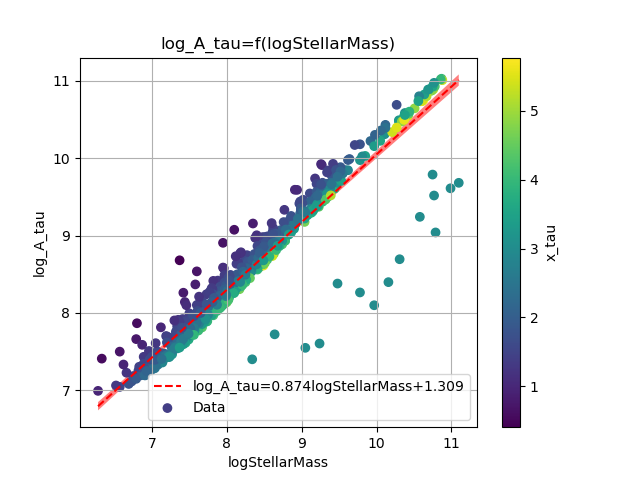
\includegraphics[width=.9\linewidth]{./figs/logStellarMass-log_A_tau-color_x_tau.png}
\caption{\label{fig:A_tau_StellarMass}Stellar Mass \(M_*\) - \(A_{del}|_{\tau}}\)}
\end{figure}



\pagebreak
\printbibliography
\end{document}